\documentclass{beamer}

\usepackage{amsmath, amssymb, hyperref, graphics, wasysym, tikz}
%\usetikzlibrary{cd}
\usepackage{mathpazo}

\AtBeginDocument{
   \DeclareSymbolFont{AMSb}{U}{msb}{m}{n}
   \DeclareSymbolFontAlphabet{\mathbb}{AMSb}}

\newcommand{\AAA}{\mathbb{A}}
\newcommand{\C}{\mathbb{C}}
\newcommand{\Z}{\mathbb{Z}}
\newcommand{\R}{\mathbb{R}}
\newcommand{\Q}{\mathbb{Q}}

\title{MAS439 Lecture 12 \\ Nullstellensatz}

\date{November 16th}

\begin{document}

\begin{frame}
\titlepage
\end{frame}


\begin{frame}{Where were we?}

We had maps $V$ and $I$ that related the geometry of affine space and ideals of $R=k[x_1,\dots, x_n]$:

\begin{center}
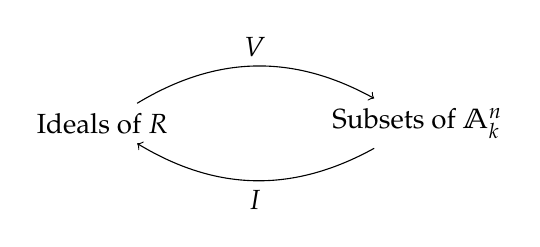
\begin{tikzpicture}

\node  (a) at (0,0) {Ideals of $R$};
\node (b) at (4,0) {Subsets of $\AAA_k^n$};

\draw[->] (a) edge[bend left] node[above] {$V$} (b);
\draw[->] (b) edge[bend left] node[below] {$I$} (a);
\end{tikzpicture}
\end{center}
Today, we're going to see how close to inverse we can make $V$ and $I$.

\end{frame}

\begin{frame}{We can't get every subset of $\AAA_k^n$}
Recall that we called a subset $X\subset \AAA_k^n$ \emph{algebraic} if $X=V(J)$ for some ideal $J$.  That is, algebraic subsets are exactly those in the image of $V$.


Since every ideal $J\subset k[x_1,\dots, x_n]$ is finitely generated, algebraic subsets were exactly those subsets that were cut out by setting a finite number of polynomials equal to 0.

\end{frame}



\begin{frame}{We can't get every ideal, either}

Let $X$ be a subset of $I$, and consider the ideal

$$I(X)=\{f\in R : f(x)=0 \forall x\in X\}$$

We note that $I(X)$ is a radical ideal, since
\begin{align*}
f^n\in I(X) & \iff f(x)^n=0\;\forall x\in X \\
&\iff f(x)=0\;\forall x \in X \\ 
& \iff f\in I(X) 
\end{align*}

\end{frame}

\begin{frame}{The best we could hope for}


\begin{center}
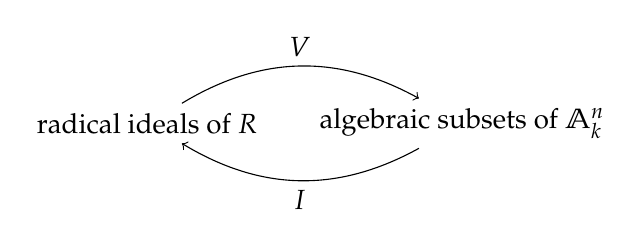
\begin{tikzpicture}

\node  (a) at (0,0) {\alert{radical} ideals of $R$};
\node (b) at (4,0) {\alert{algebraic} subsets of $\AAA_k^n$};

\draw[->] (a) edge[bend left] node[above] {$V$} (b);
\draw[->] (b) edge[bend left] node[below] {$I$} (a);
\end{tikzpicture}
\end{center}

Now it seems we have a chance...

\end{frame}

\begin{frame}{We still haven't done enough:}

Consider the following two ideals of $\R[x]$: $I=(x^2+1)$ and $J=\R[x]$ itself. \\~\\

We have $V(I)=\emptyset=V(J)$. \\~\\

Hence, $V$ is not injective, and can't have an inverse. \\~\\

\end{frame}


\begin{frame}{Another failure:}

Now, let $k=\mathbb{F}_p$, and consider the polynomial $x^p-x$. \\~\\

 Fermat's little theorem tells us that we always have $a^p\cong a\pmod p$, and hence we see that $x^p-x$ vanishes at every point of $\AAA_k^1$.  Thus, we have shown:
$$V(x^p-x)=\AAA^1_k=V(0)$$

Again, $V$ is not injective.
\end{frame}

\begin{frame}{Fixing the problem}

Both problems can be dealt with at the same time if we consider a special class of fields $k$.

\begin{definition} A field $k$ is \emph{algebraically closed} if every non-constant polynomial $f\in k[x]$ has a root in $k$.
\end{definition}

Once we have one root, we can use polynomial division and induction to show that if $k$ is an algebraically closed field then every polynomial $f\in k[x]$ can be written (uniquely, up to reordering) in the form

$$f(x)=c\cdot (x-a_1)\cdots (x-a_n)$$
for $c, a_i\in k$.


\end{frame}

\begin{frame}{Examples of fields, algebraically closed and not}

\begin{itemize}
\item $\Q$ and $\R$ are \alert{not} algebraically closed: $x^2+1$ has no roots in either.
\item $\C$ \emph{is} algebraically closed.  This is the fundamental theorem of algebra.
\item A finite field $k$ is never algebraically closed: the polynomial

$$f(x)=1+\prod_{a\in k} (x-a)$$

is not a constant, but has no roots, because $f(a)=1$ for all $a\in k$.
\end{itemize}


\end{frame}


\begin{frame}{A big word for a big theorem}

\begin{theorem}[Hillbert's \emph{Nullstellensatz}]
Let $k$ be an algebraically closed field, and $I\subset k[x_1,\dots, x_n]$ an ideal.  Then 

$$I(V(I))=\sqrt{I}$$

\end{theorem}

You will prove the Nullstellensatz next semester?

\begin{block}{A german lesson}
\begin{itemize} 
\item Null=nothing (zero)
\item Stellen=placement, location (locus)
\item satz=statement (Theorem)
\end{itemize}
so ``Nullstellensatz''= ``zero locus theorem''
\end{block}
\end{frame}


\begin{frame}{Nullstellensatz is what we needed}

\begin{theorem} Let $k$ be algebraically closed.  Then the two maps $I$ and $V$ are inverse bijections between radical ideals of $R$ and algebraic subsets of $\AAA_k^n$.
\end{theorem}

\begin{proof}
If $J$ is a radical ideal, then the Nullstellensatz says that $I(V(J))=J$.

Now, suppose $X\subset \AAA^n_k$ is algebraic; hence by definition $X=V(J)$ for some ideal $J$, which we can take to be radical.  But then 

$$V(I(X))=V(\alert{I(V(J))})=V(J)=X$$
\end{proof}
\end{frame}

\begin{frame}{An example:}

Recall your homework question, where you considered the ideal $J=(x^2+y^2-2, xy-1)$. \\~\\

Geometrically, this consists of the points $(1,1)$ and $(-1,-1)$. \\~\\

However, we saw that $(x-y)$ vanishes at both of these points, but isn't in $J$; i.e., we have  $I(V(J))\neq J$.  We did see that $(x-y)^2\in J$, consistent with $I(V(J))=\sqrt{J}$.  \\~\\

The algebraic fact that $J$ isn't radical turns out to have something to do with the fact that $V(x^2+y^2-2)$ and $V(xy-1)$ don't intersect nicely...




\end{frame}

\begin{frame}{Restricting our bijection}

Radical ideals were in bijection with algebraic subsets.  Every maximal ideal is radical -- what can we say about the algebraic subsets they correspond to?

Since $V$ and $I$ are order reversing, we see that if $\mathfrak{m}$ is a maximal ideal, then $V(\mathfrak{m}$ must be a minimal algebraic subset.  

But any point $(a_1,\dots, a_n)\in\AAA_k^n$ is algebraic, as it is $V(x_1-a_1, x_2-a_2,\dots, x_n-a_n)$.  Hence, the minimal algebraic subsets are points, and we have:

\begin{center}
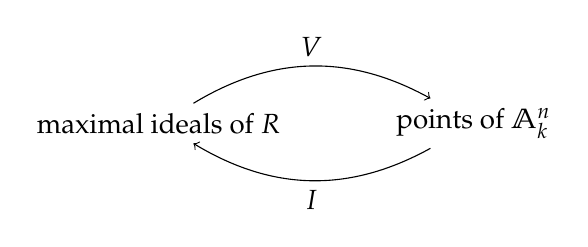
\begin{tikzpicture}

\node  (a) at (0,0) {\alert{maximal} ideals of $R$};
\node (b) at (4,0) {\alert{points} of $\AAA_k^n$};

\draw[->] (a) edge[bend left] node[above] {$V$} (b);
\draw[->] (b) edge[bend left] node[below] {$I$} (a);
\end{tikzpicture}
\end{center}

\end{frame}

\end{document}
